

%%%% Use protect on footnotes to avoid problems with footnotes in titles
%\let\rmarkdownfootnote\footnote%
%\def\footnote{\protect\rmarkdownfootnote}
%
%%%% Change title format to be more compact
%\usepackage{titling}
%
%% Create subtitle command for use in maketitle
%\providecommand{\subtitle}[1]{
%  \posttitle{
%    \begin{center}\large#1\end{center}
%    }
%}
%


\subsection{\texorpdfstring{Data simulation with
\texttt{EMtree}}{Data simulation with EMtree}}\label{data-simulation-with-emtree}

The \texttt{EMtree} package provides with simulation functions for
graphs as well as for count data under the Poisson log-Normal model.
Four types of graphs are available in the \texttt{generator\_graph()}
function: erdos (Erdös-Reyni), cluster, scale-free (from the
\texttt{huge} package) and spanning tree (from the \texttt{vegan}
package).

\begin{Shaded}
\begin{Highlighting}[]
\NormalTok{p=}\DecValTok{20}
\NormalTok{cluster=}\KeywordTok{generator_graph}\NormalTok{(p, }\DataTypeTok{graph=}\StringTok{"cluster"}\NormalTok{,}\DataTypeTok{dens=}\FloatTok{0.4}\NormalTok{, }\DataTypeTok{r=}\DecValTok{10}\NormalTok{)}
\NormalTok{erdos=}\KeywordTok{generator_graph}\NormalTok{(p, }\DataTypeTok{graph=}\StringTok{"erdos"}\NormalTok{,}\DataTypeTok{dens=}\FloatTok{0.3}\NormalTok{)}
\NormalTok{scaleF=}\KeywordTok{generator_graph}\NormalTok{(p, }\DataTypeTok{graph=}\StringTok{"scale-free"}\NormalTok{)}
\NormalTok{tree=}\KeywordTok{generator_graph}\NormalTok{(p, }\DataTypeTok{graph=}\StringTok{"tree"}\NormalTok{)}
\end{Highlighting}
\end{Shaded}

The output of \texttt{generator\_graph()} is an adjacency matrix, which
can be given as an input to \texttt{generator\_param()} to compute a
positive-definite precision matrix \texttt{omega} with signed entries,
and its corresponding variance-covariance matrix \texttt{sigma}.

\begin{Shaded}
\begin{Highlighting}[]
\NormalTok{cluster_param=}\KeywordTok{generator_param}\NormalTok{(cluster, }\DataTypeTok{signed =} \OtherTok{TRUE}\NormalTok{)}
\end{Highlighting}
\end{Shaded}

Then it is possible to simulate \texttt{n} samples of multivariate
counts under the PLN model with \texttt{generator\_PLN()}.

\begin{Shaded}
\begin{Highlighting}[]
\NormalTok{Y =}\StringTok{ }\KeywordTok{generator_PLN}\NormalTok{(cluster_param}\OperatorTok{\$}\NormalTok{sigma, }\DataTypeTok{n =} \DecValTok{100}\NormalTok{)}
\end{Highlighting}
\end{Shaded}

\begin{center}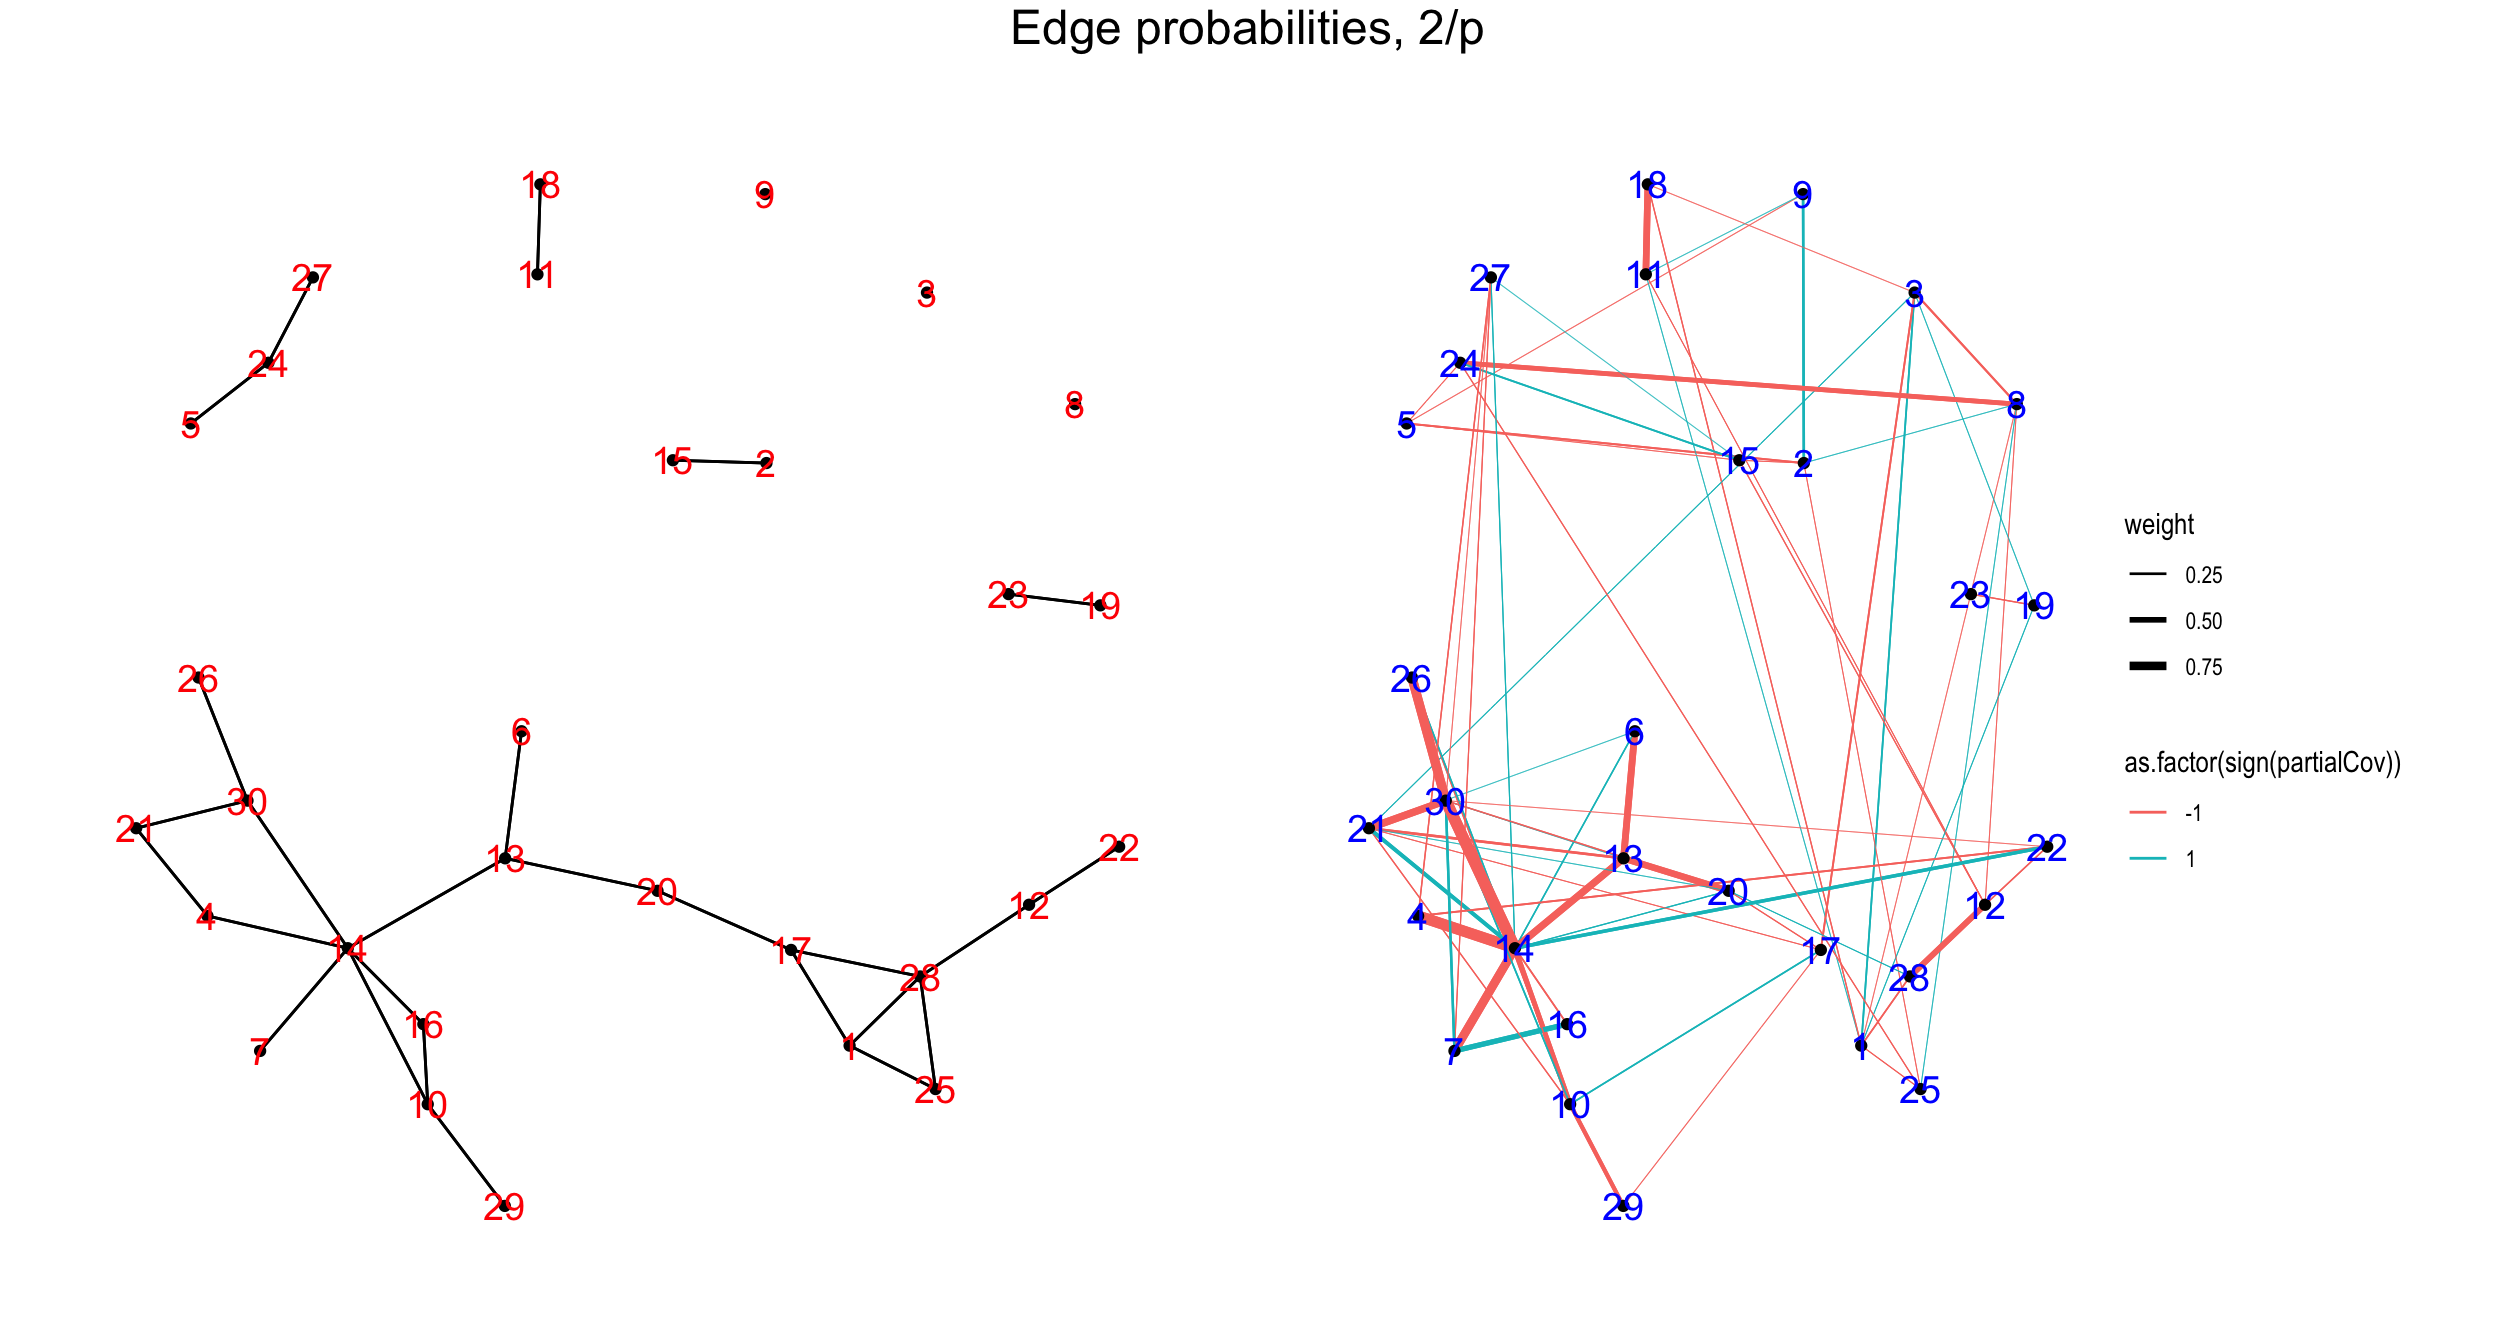
\includegraphics[width=0.5\linewidth]{EMtree/vignetteEMtree_files/figure-latex/unnamed-chunk-5-1} \end{center}

\subsection{Inference of the Fatala fishes
network}\label{inference-of-the-fatala-fishes-network}

This is a basic example detailing how to infer a network, using fishes
counts from the Fatala River (Barans95 data from the \texttt{ade4}
package).

\subsubsection{Fatala fishes dataset}\label{fatala-fishes-dataset}

The data is composed of 33 species abundances measures in 95 samples.
The available covariates are the site and date of the samples.

\begin{Shaded}
\begin{Highlighting}[]
\KeywordTok{library}\NormalTok{(ade4)}
\KeywordTok{library}\NormalTok{(tibble)}
\KeywordTok{data}\NormalTok{(baran95)}
\NormalTok{Y =}\StringTok{ }\KeywordTok{as.matrix}\NormalTok{(baran95}\OperatorTok{\$}\NormalTok{fau)}
\NormalTok{X =}\StringTok{ }\KeywordTok{as_tibble}\NormalTok{(baran95}\OperatorTok{\$}\NormalTok{plan)}
\NormalTok{n =}\StringTok{ }\KeywordTok{nrow}\NormalTok{(Y)}
\NormalTok{p =}\StringTok{ }\KeywordTok{ncol}\NormalTok{(Y)}
\end{Highlighting}
\end{Shaded}

\subsubsection{Network inference}\label{network-inference}

\texttt{EMtree} infers a network from either a correlation matrix of a
multivariate Gaussian, or an object created by PLNmodels from count
data. Therefore here we first create a \texttt{PLNmodels} object with
the \texttt{PLN()} function:

\begin{Shaded}
\begin{Highlighting}[]
\KeywordTok{library}\NormalTok{(PLNmodels)}
\NormalTok{PLNfit<-}\KeywordTok{PLN}\NormalTok{(Y }\OperatorTok{~}\StringTok{ }\NormalTok{X}\OperatorTok{\$}\NormalTok{site)}
\end{Highlighting}
\end{Shaded}

\begin{verbatim}
## 
##  Initialization...
##  Adjusting a PLN model with full covariance model
##  Post-treatments...
##  DONE!
\end{verbatim}

And then run \texttt{EMtree()}:

\begin{Shaded}
\begin{Highlighting}[]
\KeywordTok{library}\NormalTok{(EMtree)}
\NormalTok{EMtreeFit<-}\KeywordTok{EMtree}\NormalTok{(PLNfit,  }\DataTypeTok{maxIter =} \DecValTok{20}\NormalTok{, }\DataTypeTok{plot=}\OtherTok{TRUE}\NormalTok{, }\DataTypeTok{verbatim=}\OtherTok{FALSE}\NormalTok{)}
\end{Highlighting}
\end{Shaded}

\begin{center}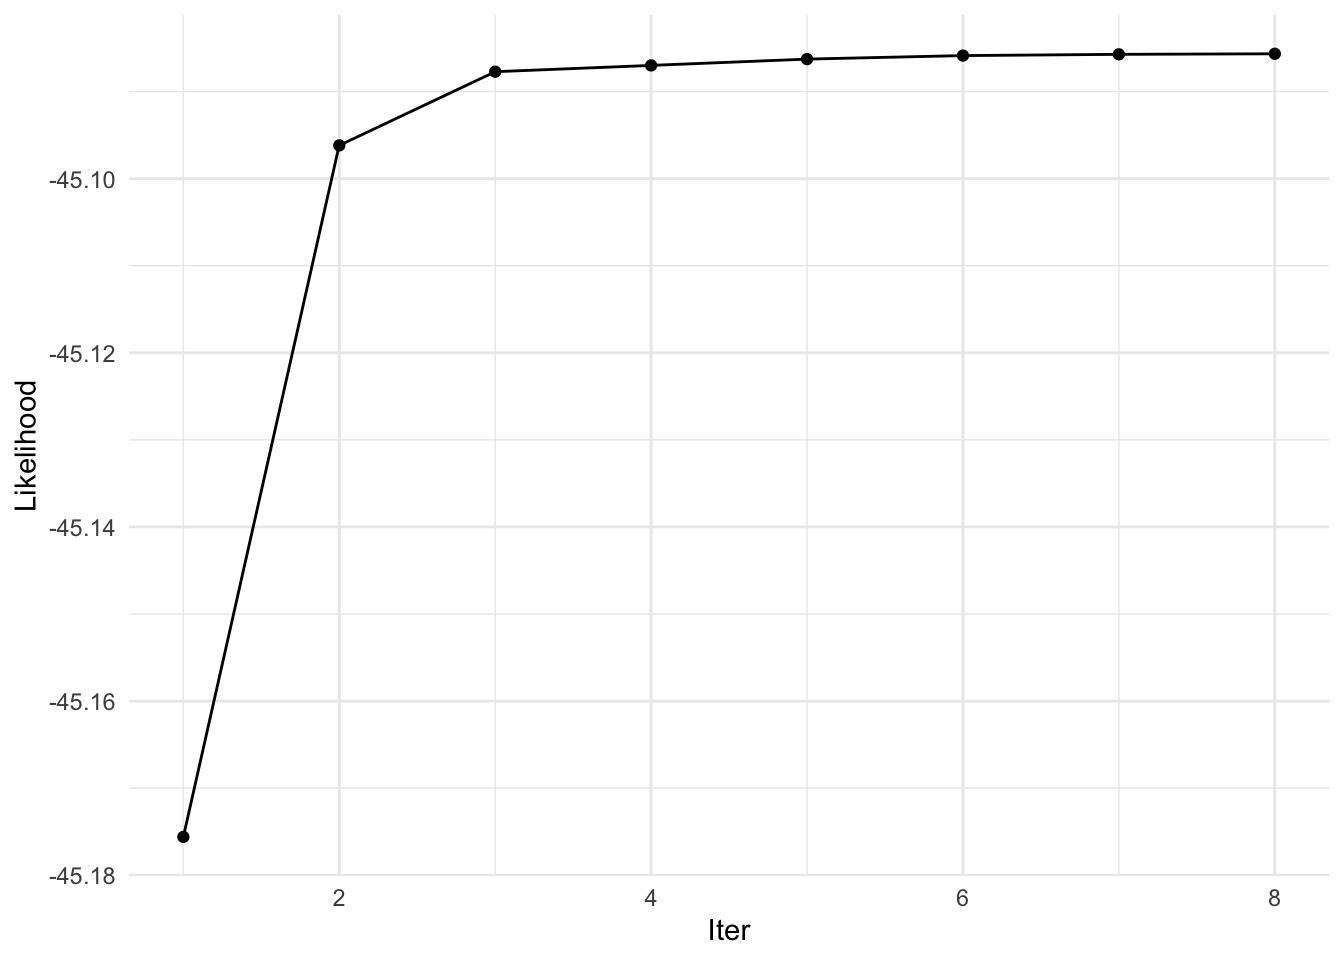
\includegraphics[width=0.5\linewidth]{EMtree/vignetteEMtree_files/figure-latex/output-1} \end{center}

\begin{Shaded}
\begin{Highlighting}[]
\KeywordTok{str}\NormalTok{(EMtreeFit)}
\end{Highlighting}
\end{Shaded}

\begin{verbatim}
## List of 6
##  $ edges_prob  : num [1:33, 1:33] 0 0.00696 0.02016 0.14686 0.03192 ...
##  $ edges_weight: num [1:33, 1:33] 0 0.000946 0.000946 0.000948 0.000947 ...
##  $ logpY       : num [1:8] -45.2 -45.1 -45.1 -45.1 -45.1 ...
##  $ maxIter     : num 8
##  $ norm.cst    : num 2.07e-50
##  $ timeEM      : 'difftime' num 0.353778123855591
##   ..- attr(*, "units")= chr "secs"
\end{verbatim}

To get a network from a fit of \texttt{EMtree()}, the probabilities
stored in \texttt{edges\_prob} can be thresholded. We suggest the
$2/p$ threshold:

\begin{Shaded}
\begin{Highlighting}[]
\NormalTok{probs<-}\StringTok{ }\NormalTok{EMtreeFit}\OperatorTok{\$}\NormalTok{edges_prob}
\NormalTok{net<-}\DecValTok{1}\OperatorTok{*}\NormalTok{(probs}\OperatorTok{>}\DecValTok{2}\OperatorTok{/}\NormalTok{p)}
\end{Highlighting}
\end{Shaded}

To improve the robstness, the function \texttt{ResampleEMtree()}
implements a statibility selection of EMtree on S sub-samples. This
function uses parallel computations with \texttt{mclapply()}. The output
\texttt{Pmat} gathers all the infered edges probabilities for each
sub-sample.

\begin{Shaded}
\begin{Highlighting}[]
\NormalTok{ResampEmtreeFit<-}\KeywordTok{ResampleEMtree}\NormalTok{(}\DataTypeTok{counts=}\NormalTok{Y, }\DataTypeTok{covar_matrix =}\NormalTok{ X}\OperatorTok{\$}\NormalTok{site , }
\DataTypeTok{S=}\DecValTok{2}\NormalTok{, }\DataTypeTok{maxIter=}\DecValTok{10}\NormalTok{,}\DataTypeTok{cond.tol=}\FloatTok{1e-8}\NormalTok{, }\DataTypeTok{cores=}\DecValTok{1}\NormalTok{)}
\end{Highlighting}
\end{Shaded}

\begin{verbatim}
## Computing  10 probability matrices with 1 core(s)...  5.78 secs
\end{verbatim}

\begin{Shaded}
\begin{Highlighting}[]
\KeywordTok{str}\NormalTok{(ResampEmtreeFit}\OperatorTok{\$}\NormalTok{Pmat)}
\end{Highlighting}
\end{Shaded}

\begin{verbatim}
##  num [1:10, 1:528] 0.01361 0.01728 0.00562 0.00348 0.00364 ...
\end{verbatim}

Edges selection frequencies can be derived from the \texttt{Pmat} output
with the function \texttt{freq\_selec()}. A final network can then be
obtained by thresholding the frequencies, to keep for example edges that
are selected in more than $80\%$ of sub-samples:

\begin{Shaded}
\begin{Highlighting}[]
\NormalTok{freqs<-}\KeywordTok{freq_selec}\NormalTok{(ResampEmtreeFit}\OperatorTok{\$}\NormalTok{Pmat,}\DataTypeTok{Pt=}\DecValTok{2}\OperatorTok{/}\NormalTok{p)}
\NormalTok{resampNet<-}\DecValTok{1}\OperatorTok{*}\NormalTok{(freqs}\OperatorTok{>}\FloatTok{0.8}\NormalTok{)}
\KeywordTok{table}\NormalTok{(net, resampNet)}
\end{Highlighting}
\end{Shaded}

\begin{verbatim}
##    resampNet
## net   0   1
##   0 873   0
##   1 112 104
\end{verbatim}

\subsubsection{Infer networks under several
models:}\label{infer-networks-under-several-models}

The aim of function \texttt{ComparEMtree()} is to run network inference
with different covariates specifications. It uses
\texttt{ResampleEMtree()} and adjust the different models specified in
\texttt{model\_names} as follows:

\begin{Shaded}
\begin{Highlighting}[]
\NormalTok{tested_models=}\KeywordTok{list}\NormalTok{(}\DecValTok{1}\NormalTok{,}\DecValTok{2}\NormalTok{,}\KeywordTok{c}\NormalTok{(}\DecValTok{1}\NormalTok{,}\DecValTok{2}\NormalTok{))}
\NormalTok{models_names=}\KeywordTok{c}\NormalTok{(}\StringTok{"date"}\NormalTok{,}\StringTok{"site"}\NormalTok{,}\StringTok{"date + site"}\NormalTok{)}
\NormalTok{compare_models<-}\KeywordTok{ComparEMtree}\NormalTok{(Y, X, }\DataTypeTok{models=}\NormalTok{tested_models, }
\DataTypeTok{m_names=}\NormalTok{models_names, }\DataTypeTok{Pt=}\DecValTok{2}\OperatorTok{/}\NormalTok{p}\NormalTok{,  }\DataTypeTok{S=}\DecValTok{3}\NormalTok{, }\DataTypeTok{maxIter=}\DecValTok{5}\NormalTok{,}\DataTypeTok{cond.tol=}\FloatTok{1e-8}\NormalTok{,}\DataTypeTok{cores=}\DecValTok{1}\NormalTok{)}
\end{Highlighting}
\end{Shaded}

\begin{verbatim}
## model date : Computing  3 probability matrices with 1 core(s)... 
##   3.68 secs
## model site : Computing  3 probability matrices with 1 core(s)... 
##   1.5 secs
## model date + site : Computing  3 probability matrices with 1 core(s)... 
##   3.95 secs
\end{verbatim}

The output of \texttt{ComparEMtree()} is a tibble in long format, which
gathers information of all interactions in all tested models.

\begin{Shaded}
\begin{Highlighting}[]
\KeywordTok{head}\NormalTok{(compare_models,}\DecValTok{4}\NormalTok{)}
\end{Highlighting}
\end{Shaded}

\begin{verbatim}
## # A tibble: 4 x 4
##   node1 node2 model weight
##   <chr> <chr> <chr>  <dbl>
## 1 1     2     date       0
## 2 1     3     date       0
## 3 2     3     date       0
## 4 1     4     date       0
\end{verbatim}

\subsection{Visuals}\label{visuals}

The \texttt{EMtree} package provides with easy plotting functions for network
visualizations. They build from the \texttt{ggraph} and
\texttt{tidygraph} packages.

\subsubsection{Simple networks}\label{simple-networks}

The function \texttt{draw\_network()} takes a weighted matrix an input,
and represent a network with edges widths proportional to the input
weights. Several layouts are available (see the \texttt{ggraph}
documentation). Nodes possessing among the highest betweenness
centrality measure can be highlighted with the parameter
\texttt{btw\_rank}.

Example from the adjacency matrices simulated earlier (cluster, spanning-tree, scale-free and erdos):

\begin{center}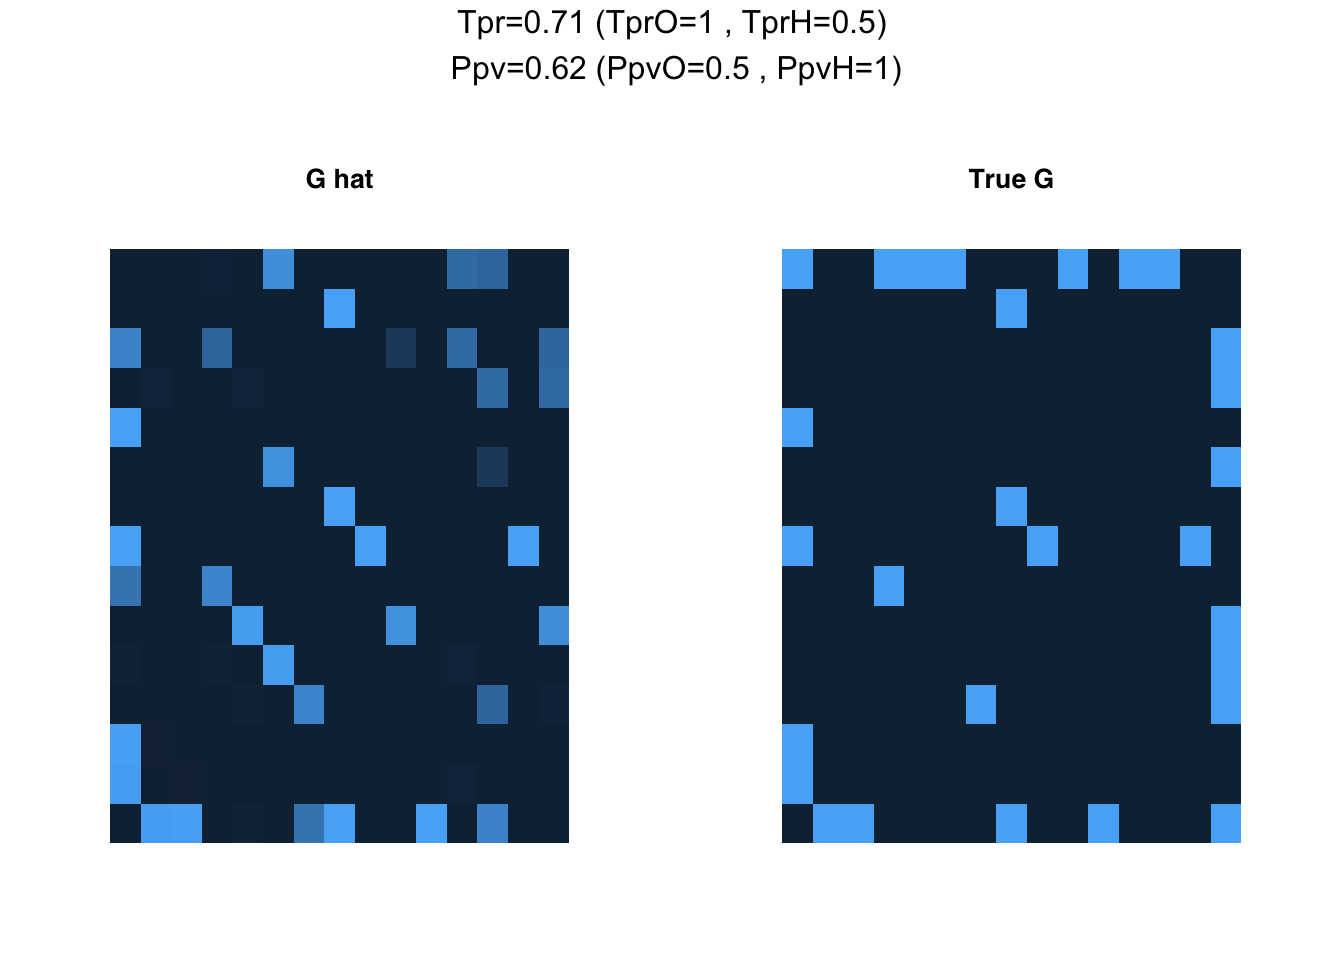
\includegraphics[width=0.8\linewidth]{EMtree/vignetteEMtree_files/figure-latex/unnamed-chunk-12-1} \end{center}

Weighted matrices can be edge probability matrices. For example, the Fatala fishes weighted network adjusted on the covariate
\textit{Site} is:

\begin{Shaded}
\begin{Highlighting}[]
\NormalTok{probs[probs}\OperatorTok{<}\DecValTok{2}\OperatorTok{/}\NormalTok{p]=}\DecValTok{0} \CommentTok{# threshold needed for representation clarity}
\KeywordTok{draw_network}\NormalTok{(probs,}\DataTypeTok{title=}\StringTok{"Site"}\NormalTok{, }\DataTypeTok{pal_edges=}\StringTok{"dodgerblue3"}\NormalTok{, }
\DataTypeTok{layout=}\StringTok{"nicely"}\NormalTok{,}\DataTypeTok{btw_rank=}\DecValTok{3}\NormalTok{)}\OperatorTok{\$}\NormalTok{G}
\end{Highlighting}
\end{Shaded}

\begin{center}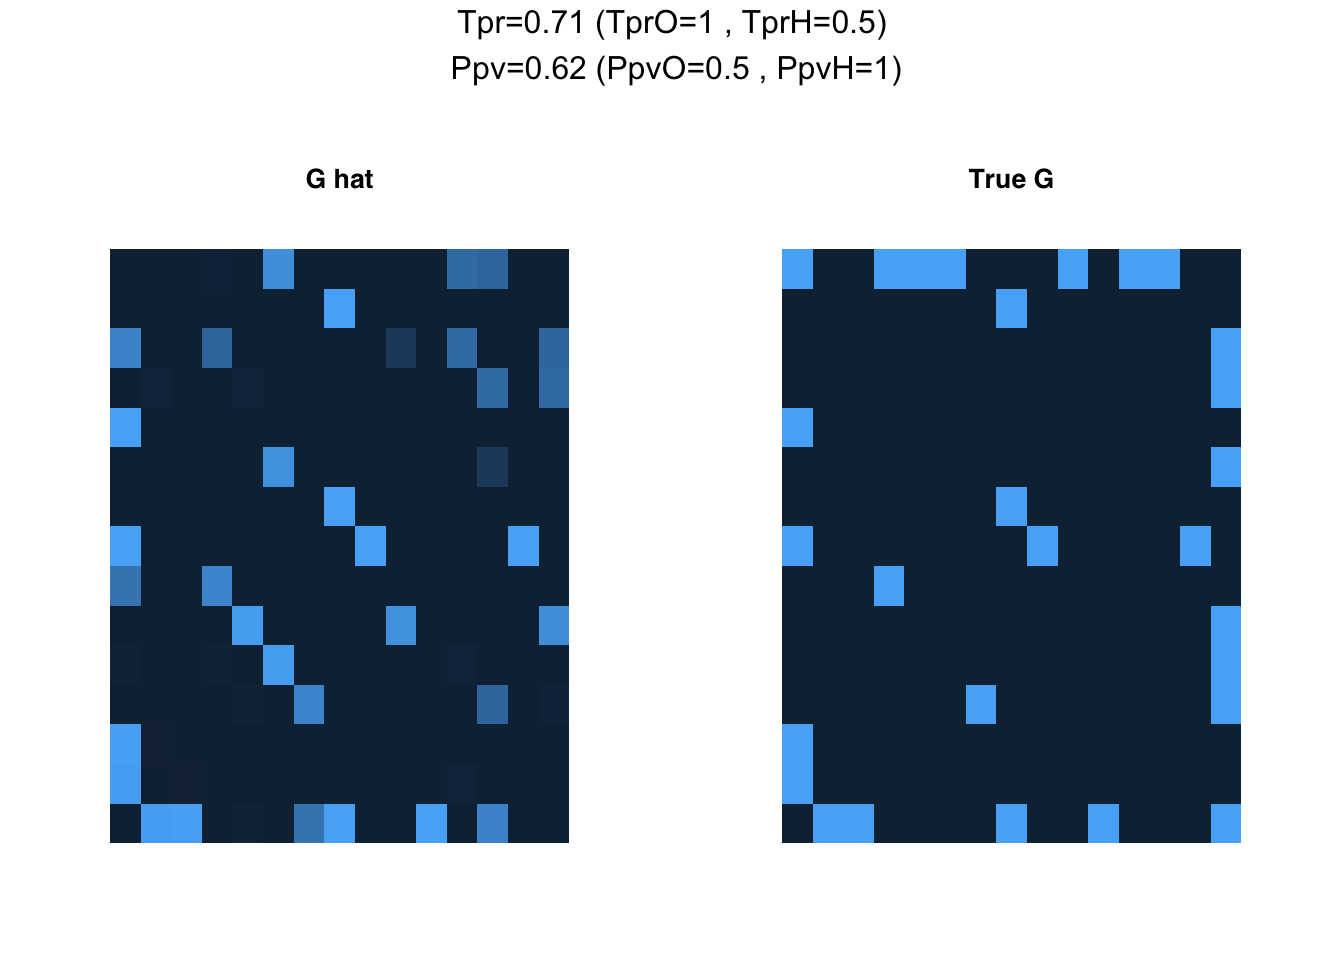
\includegraphics[width=0.5\linewidth]{EMtree/vignetteEMtree_files/figure-latex/unnamed-chunk-13-1} \end{center}

\subsubsection{Facets of several
networks}\label{facets-of-several-networks}

The function\texttt{compare\_graphs()} draws a facet plot of the output
networks from \texttt{ComparEMtree()}. Comparing network by eye is
difficult, in particular choosing the right layout to do so is often
troublesome. Here by default, the circle layout is used so that
differences in density and sensitive nodes are easily identified.

\begin{Shaded}
\begin{Highlighting}[]
\KeywordTok{compare_graphs}\NormalTok{(compare_models,}\DataTypeTok{shade=}\OtherTok{TRUE}\NormalTok{)}\OperatorTok{\$}\NormalTok{G}
\end{Highlighting}
\end{Shaded}

\begin{center}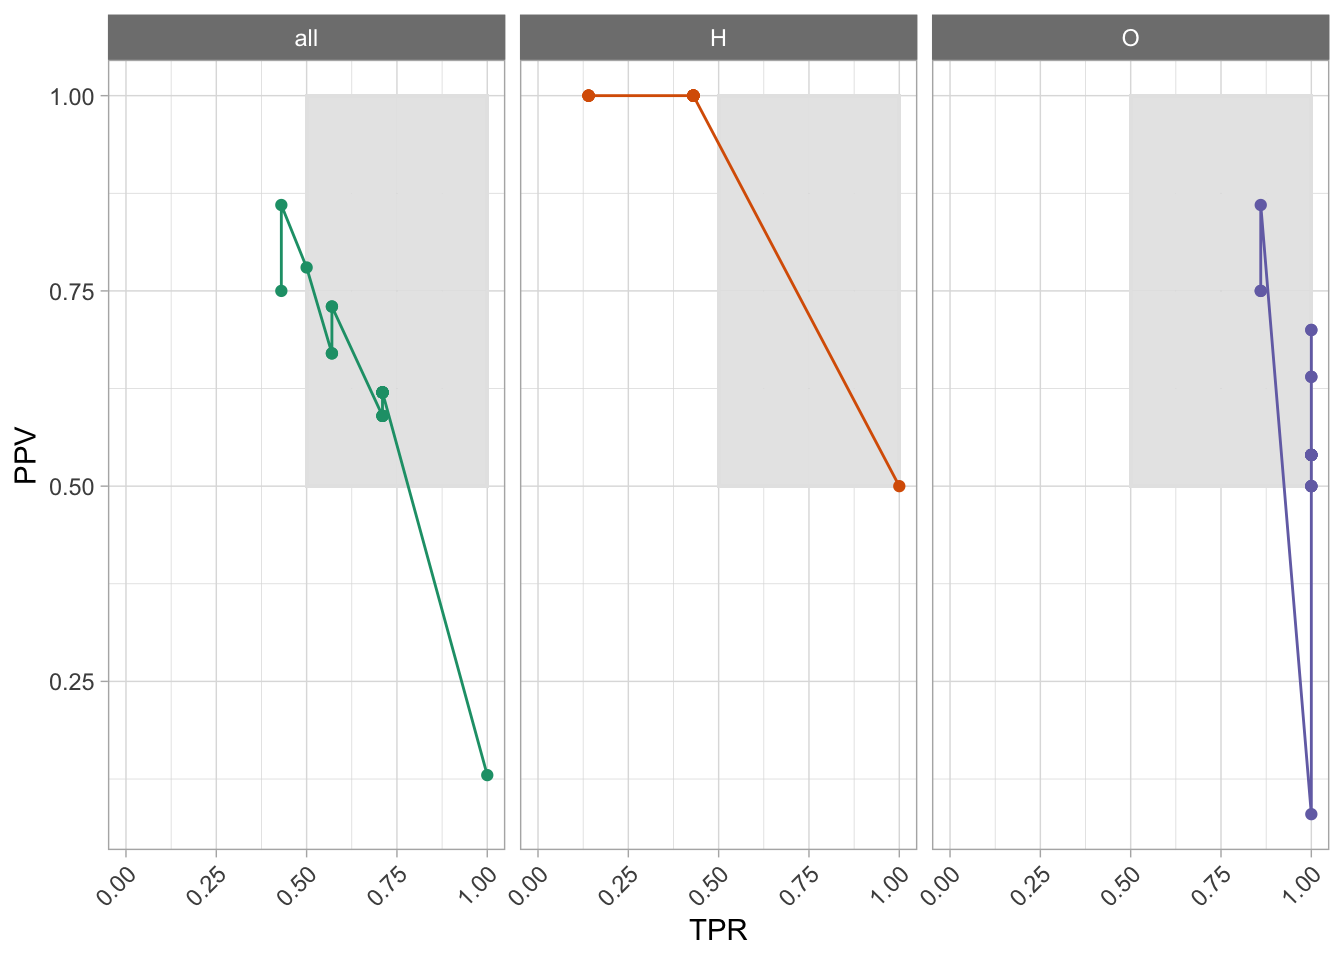
\includegraphics[width=0.8\linewidth]{EMtree/vignetteEMtree_files/figure-latex/unnamed-chunk-14-1} \end{center}

However, if another layout is preferred the nodes position is preserved
along the facet and defined by choosing the \texttt{base\_model}.

\begin{Shaded}
\begin{Highlighting}[]
\KeywordTok{compare_graphs}\NormalTok{(compare_models,}\DataTypeTok{shade=}\OtherTok{FALSE}\NormalTok{, }\DataTypeTok{layout=}\StringTok{"nicely"}\NormalTok{, }\DataTypeTok{curv=}\FloatTok{0.1}\NormalTok{, }
\DataTypeTok{base_model=}\StringTok{"site"}\NormalTok{)}\OperatorTok{\$}\NormalTok{G}
\end{Highlighting}
\end{Shaded}

\begin{center}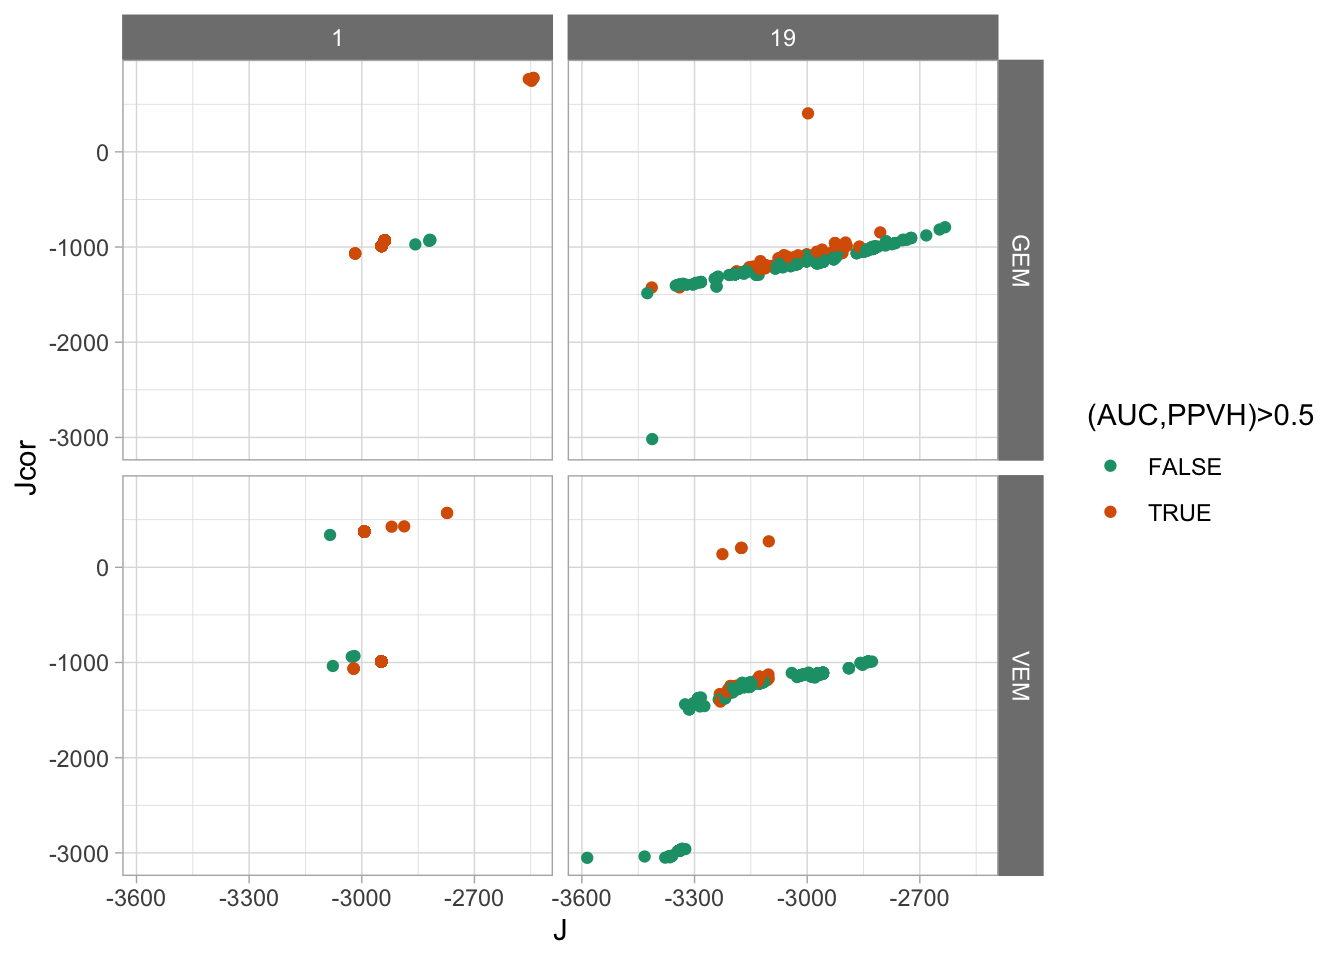
\includegraphics[width=0.8\linewidth]{EMtree/vignetteEMtree_files/figure-latex/unnamed-chunk-15-1} \end{center}

 